\documentclass{beamer}
\usetheme{Malmoe}
\usepackage{minted}
\usepackage{hyperref}


\title[Kivy]{Kivy: a sweet new app development framework}
\author[Andy Wilson]{Andy Wilson}
\date[January 2012]{January 11, 2012}

\begin{document}
%--- the titlepage frame -------------------------%
\begin{frame}[plain]
  \titlepage
\end{frame}


\begin{frame}{hey who let you in here}
I'm Andy.

Experience with mobile/desktop apps:

\begin{itemize}
  \item Kivy user since 2012
    \pause
    Saturday
    \pause
  \item I've used (and like) ETS (TraitsUI, Chaco) for numpy/scipy-type apps
  \pause
  \item Occasionally fiddle with Qt and friends (PyQT4, pyside)
  \pause
  \item I tried to do something with pygame once but got bored
  \pause
\end{itemize}
\end{frame}


\begin{frame}{the skinny}

\begin{itemize}
  \item Fast: OpenGL hardware accelerated goodness (OpenGL ES 2.0) baked in
  \pause
  \item Simple: beautiful API
  \pause
  \item Multitouchtouchtouch
  \pause
  \item Crossplatform: Linux, Windows, OSX, Android
  \pause
  ...iOS (coming soon?)
  \pause
  \item License: LGPL3
\end{itemize}

\end{frame}


\begin{frame}{howsisworkthen?}

\begin{center}
  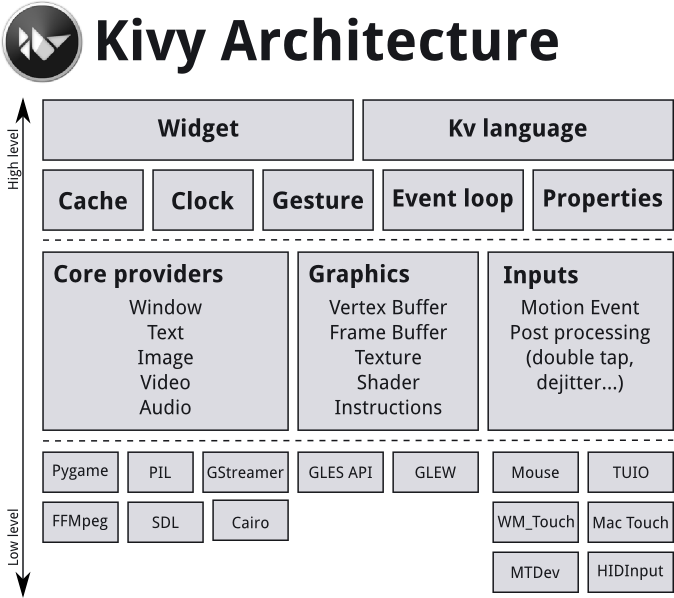
\includegraphics[height=.75\textheight]{architecture.png}
\end{center}

source: http://kivy.org/docs/guide/architecture.html

\end{frame}


\begin{frame}{widgets}
\begin{itemize}
  \item anything you touch
  \pause
  \item every kivy app has at least one root widget that takes up the whole app window/frame/screen
  \pause
  \item it's a tree!
  \pause
  \item they're great
  \pause
  \item
\end{itemize}

\end{frame}


% \begin{itemize}
%   \item
%   \pause
%   \item
% \end{itemize}

\begin{frame}{graphics}
\end{frame}

\begin{frame}[fragile]{graphics example}
  \begin{minted}[linenos]{python}
    class Foo(Widget):
        def __init__(self, **kwargs):
            super(Foo, self).__init__(**kwargs)
            with self.canvas:
                # set color
                Color(1., 0., 0.)
                # draw stuff with primitives
                Rectangle(100, 100)
  \end{minted}
\end{frame}


\begin{frame}{kivy language (.kv)}

\end{frame}


\begin{frame}{events}

\end{frame}


\begin{frame}{other nicities}
\begin{itemize}
  \item Cache
  \pause
  \item Vectors!!!
\end{itemize}
\end{frame}


\begin{frame}[fragile]{hello world}
  \inputminted{python}{hello_world.py}
\end{frame}



\begin{frame}{[CITATION NEEDED]}

Kivy project:  \url{http://kivy.org}

Source: \url{http://github.com/kivy/kivy}

Code/presentation: \url{http://github.com/wilsaj/flingy}

\end{frame}


\begin{frame}{two men enter one man leaves}

contest: \url{http://kivy.org/\#contest}

\begin{itemize}
  \item make a game
  \item use Kivy + pure python - no custom C or C extensions
  \item put it on github
  \item registration deadline is Jan 25th - contest ends Jan 31st
  \item prizes: android tablets, github subscriptions, t-shirts
\end{itemize}
\end{frame}


\end{document}